 
 \section{Seamless Migration and Dynamic NF Policy}

A separation of control plane and data plane improves the system efficiency (only small amount of logic at the data plane), facilitates the deployment (no modification of existing protocols), and reduces the implementation complexity. In this section, we first cover the port identification phase, and then explain data plane update mechanisms to achieve (1) loss-free and (2) order-preserving updates. 

\subsection{Architecture}


We first briefly cover operating systems' networking stack in \S~\ref{nks}, and then we explain our architecture design and introduce a separation of control plane and data plane. 

\subsubsection{Networking Stack} \label{nks}
Today the host's networking stack uses five-tuple to identify and route flows. Once a socket is created in the \textit{user} space, it copies the packet from \textit{user} to \textit{kernel} space to loop back or send out to a network interface. All network traffic goes through a routing table in the \textit{kernel space}, for routing decision lookup, packet filtering and/or modification. Once the kernel decides where to send, it calls an interrupt and passes the packets to the NIC driver and the driver does its job (e.g., checksum if offloaded to the driver) before finally sending out.

\begin{figure}[ht]
\centering
% 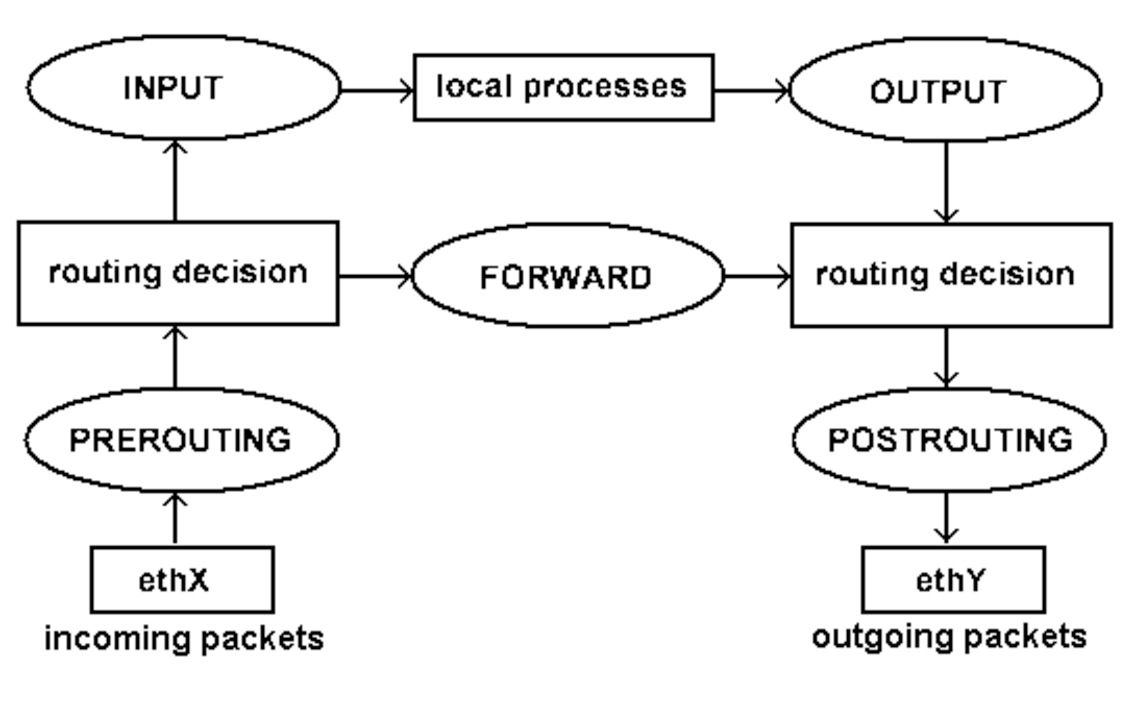
\includegraphics[scale=0.25]{figures/netfilter.pdf} 
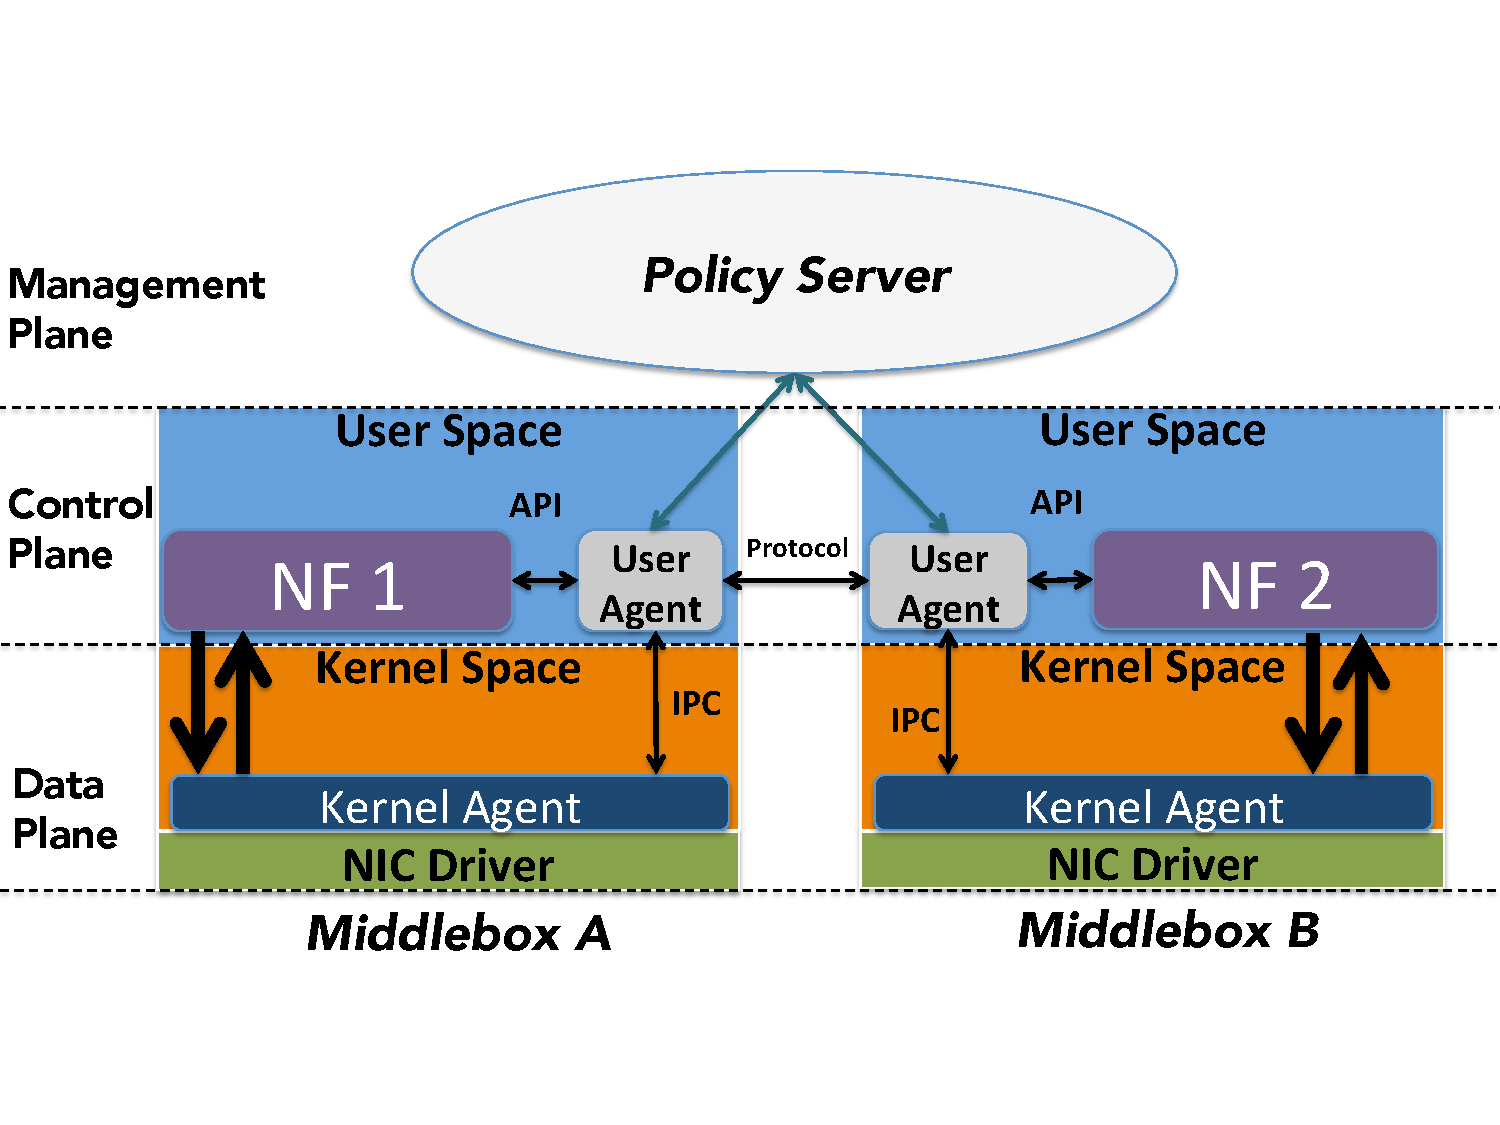
\includegraphics[width=\linewidth]{figures/architecture.pdf} 

\caption{\small System Architecture: each middlbox's user agent talks to other middlboxes, network functions, and the policy server}\label{netf}
\end{figure}

\subsubsection{Middlebox Networking System} \label{kernelagent}
Intuitively, we can implement a Middlebox Mobility Session Protocol, and port TCP and UDP to it, or revise TCP and UDP directly to support MBP. However this suffers from deployment issue. Even if IETF standardizes the protocol, it may still take a long time to integrate and widely deploy in operating systems. We also need to extend the support for all protocols (e.g., ICMP and ST).  Thus, it is important to define a set of goals before designing the system. After discussing with network researchers and operators, and learning lessons from MPTCP~\cite{MPTCP} and IPV6~\cite{IPV6}, we propose the following design principles:

\begin{itemize}
% \item the system should require minimum change in middlebox applications
\item it should not be protocol specific
\item it should have modest overhead
\item it should be non-intrusive and deployable
\end{itemize}

Based on these goals, adding functions at the bottom of Linux network stack (e.g., Netfilter~\cite{Netfilter}) or on the top NIC driver (e.g., DPDK~\cite{dpdk}) should be desirable; since (i) it can be easily installed in any Linux system with very small amount of change; (ii) it inspects all types of packets and thus not protocol specific and (iii) a kernel or driver implementation by nature has a low overhead. \amy{Confused here: isn't ``bottom of Linux network stack'' the same thing as ``on top of the NIC driver''? Basically, you are saying you want to insert a layer in between when the kernel hands packets off to the NIC driver, right?}


We choose to implement at the bottom of Linux network stack because only a limited number of hardware NIC support DPDK. Doing it at DPDK becomes more problematic when there are multiple network devices; the kernel has to decide which device to send to. 
In order to ease the complexity of implementation, we also lift most functionality up to user space. This would create a natural separation of control plane and data plane, where the control plane communicates with complex logic and the data plane only does takes actions (e.g., header rewriting, queuing to user space and kernel hash table update). We implemented a kernel agent using hook functions in Netfilter, and the functions are hooked into OUTPUT and INPUT in the client side, and all four hooks in middlebox side. The user and the kernel agent communicate via Inter-Process Call (IPC). The kernel agent has an action hash table keyed by the five-tuple. The user control agent communicate to the policy server and other middlebox control agent via UDP socket, computes and pushes updates to the kernel agent. The system consists of a kernel module and a user-level application. A brief architecture is in figure~\ref{netf}.

\begin{table}[t]\label{middleboxextension} 
\centering
 
\small
\begin{tabular} {c |c |c |c}


      Name          	  &         Type           & Key        	 &      Binding   \\
                      	  &                        &  Functions          &       Library  \\ \hline
Squid~\cite{squid} 	  &        Proxy           &  getsockopt()        & user socket  \\ \hline
PRADS~\cite{prads}	  &      Monitoring        &    got\_packet()      & libpcap~\cite{tcpdump}   \\ \hline
Bro~\cite{bro}      	  &      IDS               &   DumpPacket()      & libpcap   \\ \hline
Snort~\cite{snort}  	  &        IDS/IPS         &    PQ\_Show()          & libpcap \\ \hline
Balance~\cite{balance}	  &      Load Balancer     &    recv(), writen()       &user socket\\ \hline
Traffic   		  &    WAN-                &     net\_receive       &Linux  \\ 
Squeezer ~\cite{tsqueezer}&Optimizer &\_skb()   & skbuff \\ \hline


\end{tabular}
\caption{\small Summary of Middleboxes that we need to modify to support middlebox session protocol }
\end{table}

\subsubsection{Middlebox Support}
We also investigated a wide range of network functions to ensure the generality of our design. 

There are two possible approaches to make middlebox software to support the system: 
\begin{enumerate}
 \item \textbf{Restoring the header:} One way without modifying the middlebox is to restore the packets' super-session header. Middleboxes use the super-session header to give a verdict, e.g., monitoring or IDS. The \amy{what is the ``system''? Where exactly does header restoration happen?} system restores packets' super-session header before directing to a network function. 
 
 
 \item \textbf{Informing the network function:} Another option is to pass the mapping between the sub-session and super-session to the network function, and let the network function use the mapping. One good example here would be a transparent cache proxy~\cite{squid}, where the proxy gets the packets from its listening port and knows the final destination of the packets. 
 \amy{You use ``middlebox'' and ``network function'' interchangeably. Is this common practice? It seems a little distracting / inconsistent to me, but if this is normally done in networking papers, then I have no problem}
\end{enumerate}


There are two types of middleboxes --- active or passive functions --- based on whether it acts on the original packet. Network functions that do not act on the original packets, i.e., passive functions, mostly use libpcap to get a clone of the original packet and decide based on the copy. Libpcap captures packets at PF\_PACKET, bypasses Linux network stack, and sends the packet directly to user space. To support it, we can either bind the system with libpcap if using the first approach, or modify key functions if using the second approach. \amy{What is the first approach? What is the second approach? Do you mean passive vs active? Do you mean how network functions choose to get the packet for inspection and decision-making?} For active functions, usually packets go through network stack, and thus restoration is supported natively from the system. Sometimes the second approach is more desirable for active functions. For example, in the case of cache proxy, the sub-session terminates at the proxy and a new sub-session starts from the proxy to the server, and therefore the network function and the protocol should be aware of each other. 

\subsection{Loss-Free Update}

In the protocol design, we have suspending/suspended phases, where the system stops sending traffic for migration. However, it is hard to achieve it without modifying TCP or other protocols' control logic. We need a workaround to ensure the initial deploy-ability goal: \textit{it is network protocol independent and requires no change in existing protocols}. 

To do this, we first need to understand the control logic in these protocols: there is a hash table that tracks connection and accepts flows from established connection. If we insert a middlebox protocol, this protocol translates an original flow to its sub-sessions and translate back to the original flow for the returning traffic. Moving the flow from one path to another is equivalent to updating the translation layer at the data plane. A correct update should ensure that we do not send the traffic through the new path unless the path is set up, otherwise either side will see unexpected packets and pop up error like ``\textsf{Connection reset by peers}". 

How to find the right sequence of updates for a general network is proven to be NP-complete~\cite{SWAN, zUpdate}, but for a special topology, linear in our setting, we can apply the concept from network consistent update~\cite{consistentupdate, ratul}. We first ensure that the new configurations are all pushed before the ingress applies the new configuration, and the old configurations are not removed until the egress sends the last packet. In particular, when a migration is initialized from the middlebox, it notifies its neighbor, which inserts a new translation rule for incoming traffic. Then this neighbor notifies the other side of the connection via UPDATE-SYN. Each hop receiving UPDATE-SYN updates its own translation table. Once the target host receives the notification, the new configuration will have been installed at every hop for one direction of the traffic, and thus we apply the new configuration for all new packets after the greatest sequence number seen so far. The opposite direction is set up via the same way from UPDATE-SYN-ACK. Once the old connection sees no packet for a certain period of time, e.g. a timeout, we remove the old configuration using the same mechanism. 

\textbf{Theorem:} 
The update is per-packet consistent. 

\begin{proof}
We prove by reducing the problem to a generalized consistent update~\cite{consistentupdate}. We build the case where the network has a linear topology, and each flow with five tuples has a unique rule, then the update approach is two-phase update. A two-phase update ensures per-packet consistency. 
 
\end{proof}

\begin{figure}[ht]
\centering
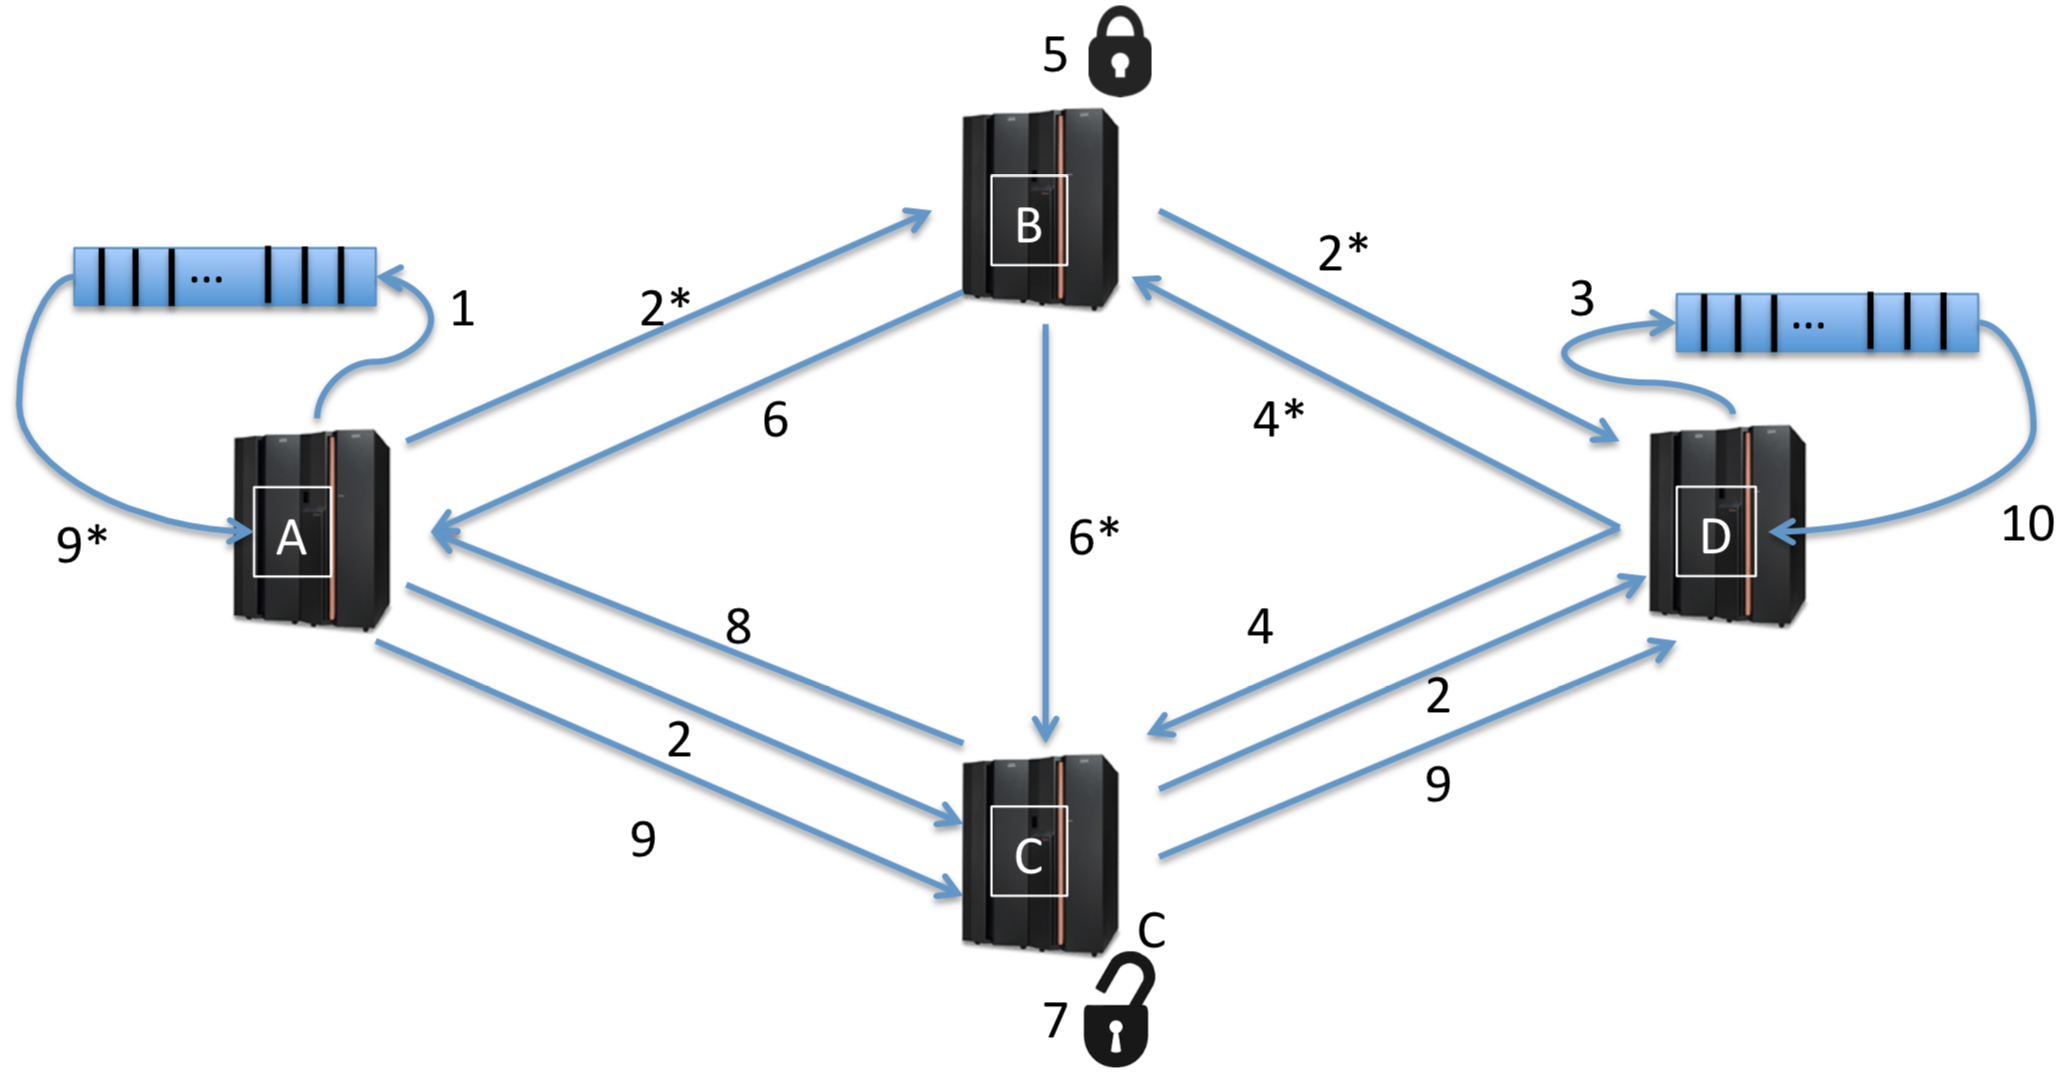
\includegraphics[width=\linewidth]{figures/order_preserving.png} 

\caption{\small We assume the migration is initiated at middlebox D, and the steps for an order-preserving update: 1. lock outgoing traffic; 2. send SYN packets; 3. lock the reverse direction traffic; 4. send SYNACK packets; 5. lock middlebox states; 6*. migrate states; 6. send SYNACK from old path; 7. finish migration and unlock states; 8. send SYNACK from new path; 9*. release buffered traffic; 9. send ACK packets; 10. release buffered traffic from the other side}\label{orderpreserving}
\end{figure}

\subsection{Traffic-Locking Update}

In a loss-free update, we keep traffic on the old path before the new path is set up. However, we may fail to migrate the flow, since this requires us to migrate middlebox state but the state cannot be moved since it is being continuously updated as the packets coming in. In this case, to lock and migrate the middlebox state we should stop sending traffic during the new path setup. Since changing the protocols (e.g., TCP and UDP) flow control logic is undesirable, we choose to buffer the traffic and not to release it until the middlebox state on the old path has been locked and replicated to the new middlebox. A fully described migration is in figure~\ref{orderpreserving}.


The definition for \textit{an order-preserving update} is that the update itself does not introduce reordering. A traffic-locking update is also order-preserving. If we assume a FIFO network with no congestion, the protocol control messages are sent after the locking of the flow, and thus it comes after the last packet sent on the path. It is safe to lock and migrate middlebox states after seeing the SYNACK packet because this packet signals both directions are locked, and thus is after the last packet sent from both directions. The update mechanism does not break the initial network semantics. (Note the mechanism does not guarantee order-preserving if the network is not FIFO or loss-free.) 

\begin{figure}[ht]
\centering
% 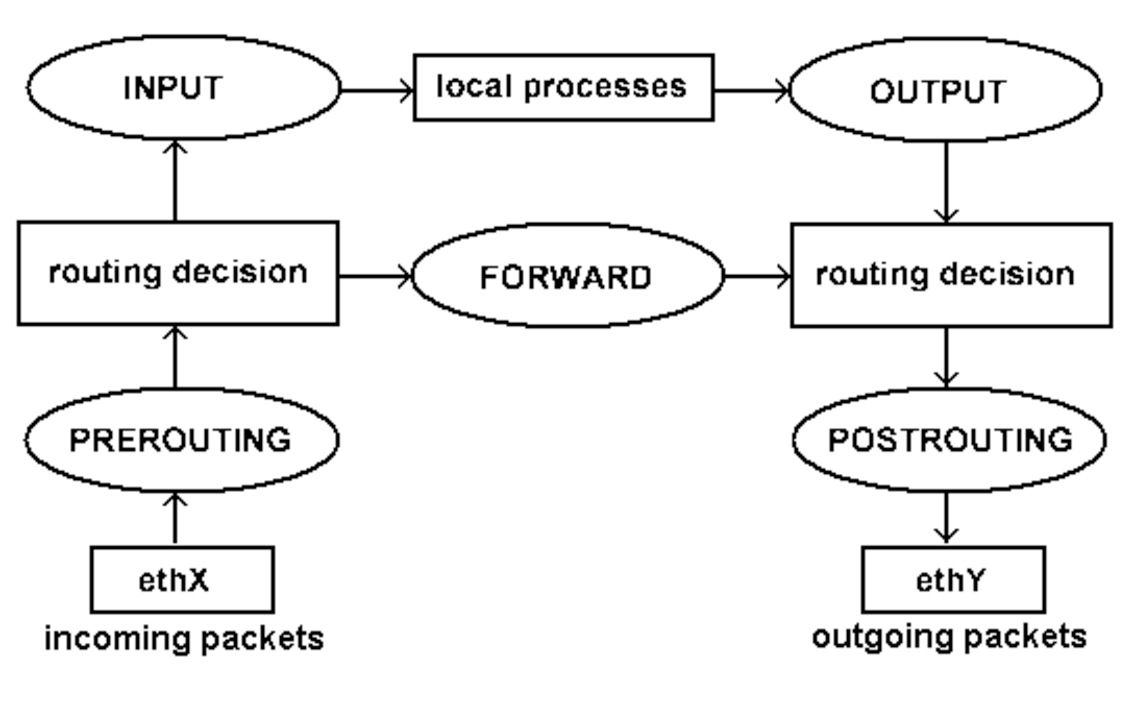
\includegraphics[scale=0.25]{figures/netfilter.pdf} 
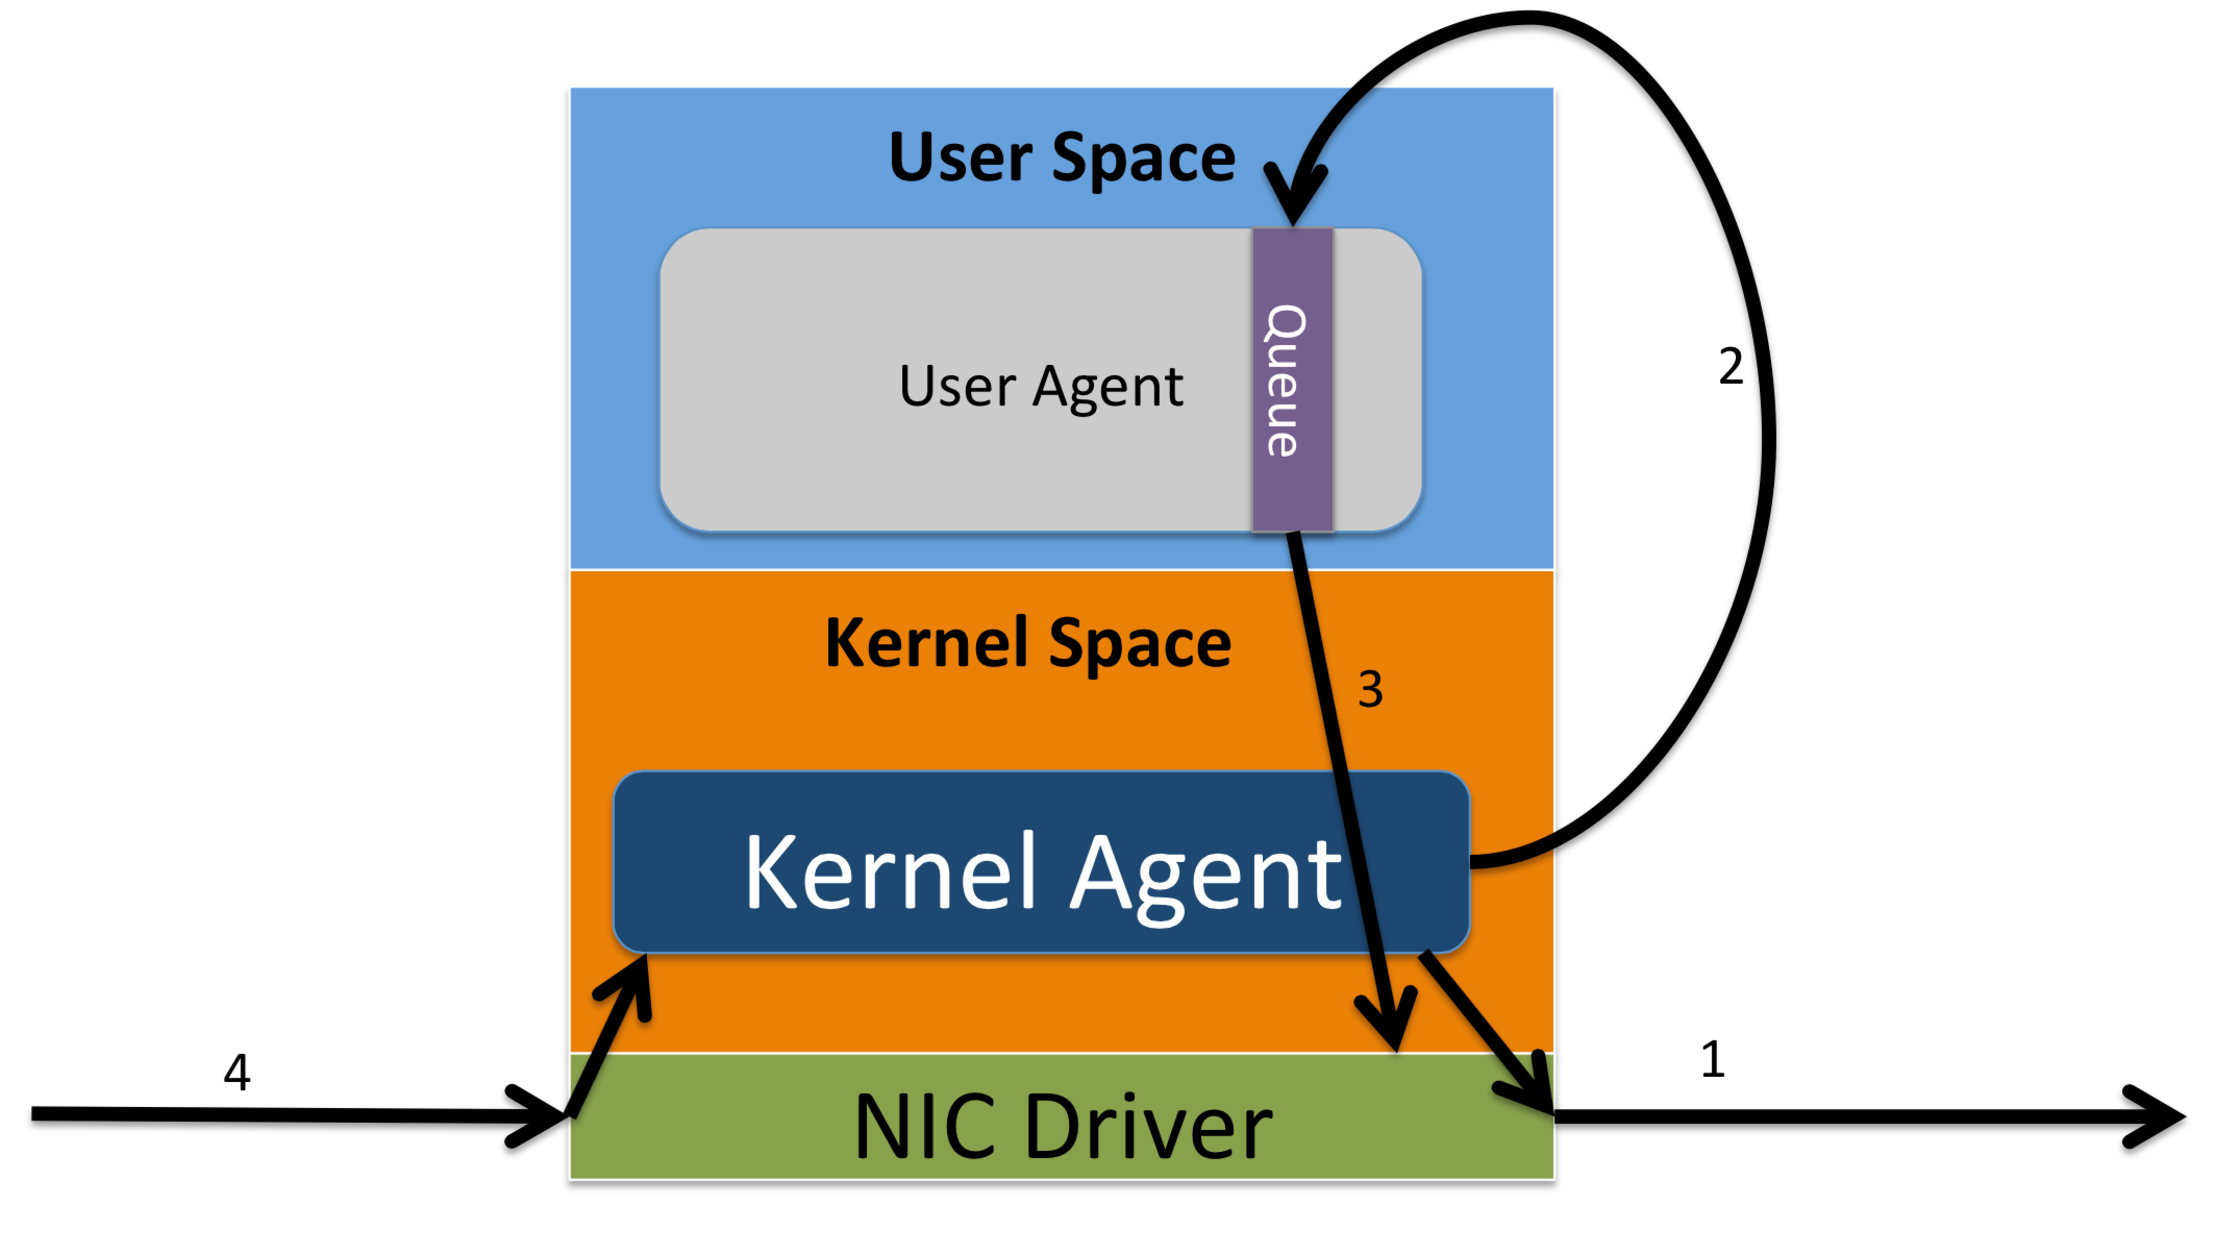
\includegraphics[width=\linewidth]{figures/flowstream.pdf} 

\caption{\small Data stream during order preserving migration: the system 1. sends out traffic through the old path, 2. buffers the packets in the user space queue, 3. receives notification from the other side and releases the buffer, and 4. directs newly coming traffic through the new path}\label{flowstream}
\end{figure}




\begin{algorithm} [ht]
\small
\SetAlgoLined

\SetKwFunction{packet}{packet\_out}\SetKwFunction{IPC}{command\_in}\SetKwFunction{queue}{Queue Agent}
\SetKwProg{mypacket}{Event\_Handler}{}{}
\SetKwProg{func}{Program}{}{}

\mypacket{\packet{} } {
lock\;
action lookup\;
\If{During Migration}{
\If{Buffer is needed}{
unlock\;
send to user queue\;
}\Else {
  \emph{Note: we do not unlock here, wait for queue to drain}\;
  mark the last packet\;
  send to user queue\;
  
  Migration = False\;
  }
} \Else{ 
  unlock\;
  send out\;
  }
  }
\mypacket{\IPC{} } {
  \If{MBP.SYN\_Update==True}
  {
  Migration = True\;
  ToBuffer = True\;
  }
  \If{MBP.ACK\_Update==True}{
  ToBuffer = False\;}
  \If{User queue is drained}{
  unlock\;
  } 
}
\func{\queue{}} {
  \If{MBP.ACK\_Update==False}{
  wait\;
  }  \Else{
    \While{queue is not empty}{
    send out\;
    \If{marked as the last packet}{
    notify kernel queue is drained\;
    }
    }
  }

} 
\caption{Order Preserving Flow Migration} \label{sync}

\end{algorithm} 


There is one more issue here we need to address: since at the high traffic rate we can only queue packets in the user space, we have an issue of synchronization between the user space queue and kernel space flow. In figure~\ref{flowstream} step 3 and step 4 may be interleaved, which breaks the initial network semantics. One solution is to keep the queue and enqueue all packets, however this severely penalizes the general case where the system is not in an update phase. To address this issue, we decide to take advantage of the spin\_lock for the hash table lookup, and lock the packet\_out interrupt if the user queue is not drained yet. A complete algorithm is in algorithm~\ref{sync}, and to add concurrency, we can have a flow to lock for each flow and add another lock lookup beforehand. 



\begin{comment}
\begin{algorithm} [ht]
\tiny
\SetAlgoLined
\SetKwFunction{packet}{packet\_out}\SetKwFunction{IPC}{command\_in}
\SetKwProg{mypacket}{Event\_Handler}{}{}
\mypacket{\packet{} } {

\nl Lock()\;
\nl action lookup\;
\nl Send\_out()\;
\nl Unlock()\;
}
\mypacket{\IPC{} } {
  \If{MBP.SYN\_Update==True}
  {
  \nl Lock()\;
  \nl Update action\;
  }
  \If{MBP.ACK\_Update==True}{
  \nl Unlock()\;
  } 
}

\caption{A naive solution} \label{wrongalgorithm}
\end{algorithm} 

A naive solution like algorithm~\ref{wrongalgorithm} should guarantee the synchronization in theory. However, it does not work well in practice, since interrupt-disallowed spin lock would lock the thread in the top half of Linux kernel, this can be very problematic if we have long update or timeout (e.g., $>100 ms$ ), and the NIC may drop the packets if they are not handled by kernel in time, to accept new packets.
\end{comment}


